%% Determines the type of document (including standard settings for layout).
\documentclass[letterpaper]{article}



%% Package to control the size of a page: the standard margins used by LaTeX are
%% very wide!
\usepackage[margin=1in]{geometry}


%% Packages add functionality to the document. The AMS packages are standard
%% packages to support various mathematical notations. AMS stands for American
%% Mathematical Society, the organization that maintains these packages.
\usepackage{amsmath,amsthm,amssymb}

%% Theorems-like environments using functionality provided by amsthm.
\theoremstyle{plain}
\newtheorem{theorem}{Theorem}[section]
    %% [section] at the end specifies that theorems should be numbered
    %% per-section: Section x starts with theorem-like x.1 and so on, ...
\newtheorem{proposition}[theorem]{Proposition}
    %% [theorem] in the middle specifies: use the same counter as the theorem
    %% environment: here we number all theorem-like environments consecutively.
\newtheorem{corollary}[theorem]{Corollary}
\newtheorem{lemma}[theorem]{Lemma}
\theoremstyle{definition}
\newtheorem{definition}[theorem]{Definition}
\theoremstyle{remark}
\newtheorem{example}[theorem]{Example}
\newtheorem{remark}[theorem]{Remark}


%% Support for nicely formatted tables.
\usepackage{booktabs}


%% Support for colors & colors in tables.
\usepackage[table]{xcolor}

% Seven colors safe for use color blindness.
% Colors taken from doi:10.1038/nmeth.1618.
\definecolor{cbOrange}{RGB}{230,159,0}
\definecolor{cbSkyBlue}{RGB}{86,180,233}
\definecolor{cbBluishGreen}{RGB}{0,158,115}
\definecolor{cbYellow}{RGB}{240,228,66}
\definecolor{cbBlue}{RGB}{0,114,178}
\definecolor{cbVermillion}{RGB}{213,94,0}
\definecolor{cbReddischPurple}{RGB}{204,121,167}


%% Notation used in this document.
\newcommand{\n}{\mathbf{n}} %% Num. Replicas.
\newcommand{\f}{\mathbf{f}} %% Num. Faulty Replicas.

%% Misc. Math notation.
\newcommand{\BigO}{\mathcal{O}}
\newcommand{\abs}[1]{\lvert #1 \rvert}
\newcommand{\AName}[1]{\textsc{#1}}
\newcommand{\Var}[1]{\texttt{#1}}


%% Algorithms.
\usepackage{algorithm}
\usepackage[noend]{algorithmic}
\newcommand{\GETS}{:=}


%% Formatting SI-units.
\usepackage{siunitx}
\sisetup{per-mode=symbol}


%% TikZ: for creating figures.
\usepackage{tikz}

%% Configuration for figures: Nicer arrows.
\usetikzlibrary{arrows.meta}
\tikzset{>=Stealth}
\usetikzlibrary{automata,positioning,arrows}


%% pgfplots: drawing plots using TikZ.
\usepackage{pgfplots}
%% Configuration for plots: Use color-blind friendly colors.
\pgfplotscreateplotcyclelist{cbSafeList}{
    very thick,solid,cbOrange,every mark/.append style={solid},mark=*\\
    very thick,solid,cbSkyBlue,every mark/.append style={solid},mark=*\\
    very thick,solid,cbBluishGreen,every mark/.append style={solid},mark=*\\
    very thick,solid,cbYellow,every mark/.append style={solid},mark=*\\
    very thick,solid,cbBlue,every mark/.append style={solid},mark=*\\
    very thick,solid,cbVermillion,every mark/.append style={solid},mark=*\\
    very thick,solid,cbReddischPurple,every mark/.append style={solid},mark=*\\
    very thick,solid,black,every mark/.append style={solid},mark=*\\
}
\pgfplotsset{
    legend style={font=\small},
    compat=1.16,
    width=260pt,
    height=140pt,
    legend cell align=left,
    xlabel near ticks,
    ylabel near ticks,
    every axis/.append style={
        cycle list name=cbSafeList,
        ymin=0,
        enlargelimits=0.05,
        mark size=1pt,
        ylabel style={align=center},
        xlabel style={align=center},
        title style={align=center}
    }
}

%% PgfplotsTable: loading data files to use with pgfplots.
\usepackage{pgfplotstable}


%% Support for hyperlinks and urls. The setting ``colorlinks'' sets how links
%% are shown in the document (with a color, without underline). We put hyperref
%% last---it has a tendency to break other packages when loaded before them.
\usepackage[colorlinks]{hyperref}
\usepackage{graphicx}
\usepackage{pgffor}
\usepackage{caption}
\usepackage{tabularx}
\usepackage{enumitem}
\usepackage{fancyhdr}

\title{COMPSCI 2AC3 Assignment 3}
\author{Luca Mawyin - 400531739}
\date{\today}

\begin{document}

\maketitle

\section{}

\begin{align*}
    A &= \{a^n~|~n=2pq~\text{where}~p,q~\text{are prime numbers}\}
\end{align*}

Suppose the demon chooses k. We will pick $x=z=\epsilon$ and $y=a^k$. Then $xyz=a^k\in{A}$ and $|y|=k\geq{k}$. Now suppose the demon chooses $u,v,w$ of lengths $j,m,n$:
\begin{align*}
    x&=\epsilon\\
    y&=a^k\\
    z&=\epsilon\\
    |y|&=k\\
    |u|,|v|,|w|&=j,m,n\\
    k&=2pq=j+m+n,~m>0\\
    y&=uvw=a^{j+m+n}\\
    |xuv^iwz|&=j+im+n\\
    &=j+im-m+m+n\\
    &=j+m+n+m(i-1)\\
    &=k+m(i-1)
\end{align*}
We must choose an $i$ such that $k+m(i-1)\neq{2pq}$ where $p,q$ are prime numbers. Let $i=2$:
\begin{align*}
    i&=2\\
    |xuv^2wz|&=k+m(2-1)\\
    &=k+m\\
    &=2pq+m
\end{align*}
Because $m>0$, this breaks the condition of the length of the string due to the interference of $m$ being added, and therefore will result in instances where $2pq+m\neq2p'q'$. For example if $p=q=5$ and $m=1$, the string length becomes invalid as $2\times5\times5+1=51$ which cannot be expressed as $2p'q'$. Therefore, the language is not regular.

\newpage

\section{}

\begin{align*}
    M&=(Q,\Sigma,\delta,s,F)\\
    |w|&=2k\\
    w&=yuvx\in{M},~u\neq\epsilon,~v\neq\epsilon\\
    z&=yvux\in{M}
\end{align*}

As $|w|=2k$, the number of states visited, including the start state, is equal to $2k+1$. Furthermore, as $|w|>k$, this means that there are states that are visited multiple times. We will consider the first half of the states visited:
\begin{align*}
    \exists~(0\leq{i}\leq{j}\leq{k})\implies{q_i=q_j}
\end{align*}
Then, we can define a $u\neq\epsilon$ as:
\begin{align*}
    u&=a_{i+1}a_{i+2}\dots{a_j}
\end{align*}
Now we will consider the second half of the states:
\begin{align*}
    \exists~(k\leq{r}\leq{s}\leq{2k})\implies{q_r=q_s}
\end{align*}
Where $v\neq\epsilon$ can be defined as:
\begin{align*}
    v&=a_{r+1}a_{r+2}\dots{a_s}
\end{align*}
We will also define $y$ and $x$ as the strings that occur before and after $uv$, respectively:
\begin{align*}
    y&=a_0a_1\dots{a_i}\\
    x&=a_{s+1}a_{s+2}\dots{a_{2k}}
\end{align*}
As both $u$ and $v$ correspond to loops of states within M, this means that $z=yvux$ is also a valid sting in $M$ as swapping them does not change the DFA pass outside of the loops occuring for $u$ and $v$. This means that reading $z$ will still pass along valid transitions along the DFA.
\newpage
\section{}

\begin{tabular}{c | c c}
    & a & b\\
    \hline
    0F & 2 & 0 \\
    1 & 0 & 1 \\
    2F & 3 & 4 \\
    3 & 0 & 1 \\
    4F & 3 & 2 \\
\end{tabular}\\[1em]
Marking all pairs with one accept state and one nonaccept state:\\[1em]
\begin{tabular}{c c c c c c}
0 &   &   &   &   &   \\
\checkmark & 1 &   &   &   &   \\
- & \checkmark & 2 &   &   &   \\
\checkmark & - & \checkmark & 3 &   &   \\
- & \checkmark & - & \checkmark & 4 &   \\
\end{tabular}\\[1em]
Pass 2:\\[1em]
\begin{tabular}{c c c c c c}
0 &   &   &   &   &   \\
\checkmark & 1 &   &   &   &   \\
\checkmark & \checkmark & 2 &   &   &   \\
\checkmark & - & \checkmark & 3 &   &   \\
\checkmark & \checkmark & - & \checkmark & 4 &   \\
\end{tabular}\\[1em]
This means that $1\approx3\land2\approx4$. Now we will represent the minimized DFA:
\begin{center}
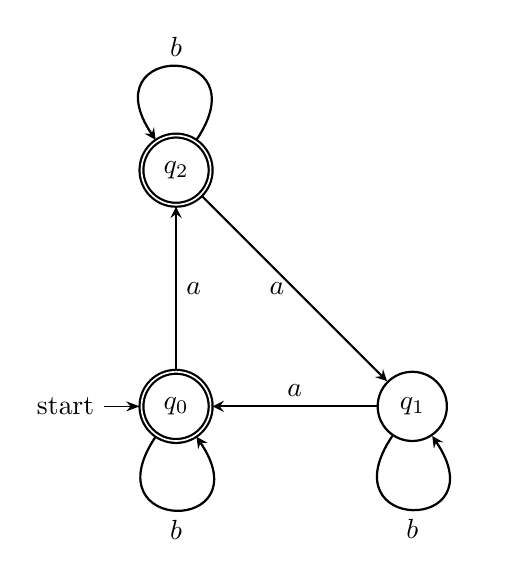
\begin{tikzpicture}[]
    \node[initial,thick,accepting,state] at (-6.5,0) (2c8c90fb) {$q_0$};
    \node[thick,state] at (-3.5,0) (6c912c23) {$q_{1}$};
    \node[thick,accepting,state] at (-6.5,3) (11ee0127) {$q_{2}$};
    \path[->, thick, >=stealth]
    (2c8c90fb) edge [loop,min distance = 1.5cm,below,in = -56, out = -124] node {$b$} (2c8c90fb)
    (2c8c90fb) edge [right,in = -90, out = 90] node {$a$} (11ee0127)
    (6c912c23) edge [above,in = 0, out = 180] node {$a$} (2c8c90fb)
    (6c912c23) edge [loop,min distance = 1.5cm,below,in = -56, out = -124] node {$b$} (6c912c23)
    (11ee0127) edge [left,in = 135, out = -45] node {$a$} (6c912c23)
    (11ee0127) edge [loop,min distance = 1.5cm,above,in = 124, out = 56] node {$b$} (11ee0127)
    ;
\end{tikzpicture}
\end{center}

\newpage

\section{}
\begin{align*}
    A&=\{0^n\alpha1^{2n}~|~n\geq{0},~\alpha\in\{0,1\}^*~\text{is a palindrome}\}
\end{align*}
We will define our CFL as $G=(N,\Sigma,P,S)$, where:
\begin{align*}
    N&=\{S,T\}\\
    \Sigma&=\{0,1\}\\
    P&= 
    \left\{
    \begin{array}{l}
       S \to T~|~0S11, \\
       T \to \epsilon~|~0~|~1~|~0T0~|~1T1
    \end{array}
    \right.
\end{align*}

\end{document}